% !TeX spellcheck = cs_CZ
%{\tikzset{external/prefix={tikz/FYZI/}}
% \tikzset{external/figure name/.add={ch19_}{}}
%---------------------------------------------------------------------------------------------------
% file fey1ch19.tex
%---------------------------------------------------------------------------------------------------
%=========================== Kapitola: Hmotný střed; Moment setrvačnosti ==========================
\chapter{Hmotný střed; Moment setrvačnosti}\label{fyz:IchapXIX}
\minitoc
  \section{Vlastnosti hmotného středu}\label{fyz:IchapXIXsecI}
  \section{Poloha hmotného bodu}\label{fyz:IchapXIXsecII}
  \section{Určení momentu setrvačnosti}\label{fyz:IchapXIXsecIII}
  \section{Kinetická energie rotace}\label{fyz:IchapXIXsecIV}
  \section{Příklady a cvičení}\label{fyz:IchapXIXsecV}

  \begin{figure}[ht!] %\ref{fyz_fig402}
    \centering
    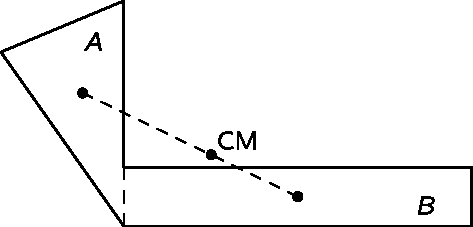
\includegraphics[width=0.3\linewidth]{fyz_fig402.pdf}
    \caption{Hmotný střed složeného tělesa leží na přímce spojující hmotné středy obou částí
             (\cite[s.~260]{Feynman01})}
    \label{fyz_fig402}
  \end{figure}

  \begin{figure}[ht!] %\ref{fyz_fig403}
    \centering
    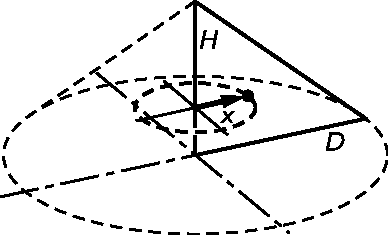
\includegraphics[width=0.3\linewidth]{fyz_fig403.pdf}
    \caption{Pravoúhlý trojúhelník a přímý rotační kužel vytvořený rotujícím trojúhelníkem 
             (\cite[s.~263]{Feynman01})}
    \label{fyz_fig403}
  \end{figure}
  \begin{figure}[ht!] %\ref{fyz_fig404}
    \centering
    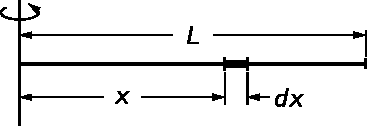
\includegraphics[width=0.3\linewidth]{fyz_fig404.pdf}
    \caption{Přímá tyč \(L\) rotující kolem osy procházející jedním koncem
             (\cite[s.~264]{Feynman01})}
    \label{fyz_fig404}
  \end{figure}

  \begin{figure}[ht!] %\ref{fyz_fig405}
    \centering
    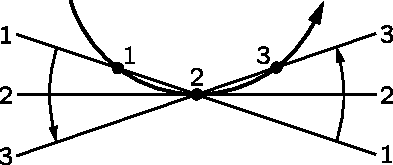
\includegraphics[width=0.3\linewidth]{fyz_fig405.pdf}
    \caption{Tři postupné pohledy na radiálně se pohybující bod na otáčející se podložce
             (\cite[s.~269]{Feynman01})}
    \label{fyz_fig405}
  \end{figure}
  
%} %tikzset
%---------------------------------------------------------------------------------------------------
\printbibliography[title={Seznam literatury}, heading=subbibliography]
\addcontentsline{toc}{section}{Seznam literatury}